% chapter_hito1.tex
%
% Hito I (27 de septiembre de 2026). Supuestos del modelo para la calibracion
% empirica del caso CORFO--Intermediario--MiPyME--Banco.
% Texto del documento del Hito I, adaptado a capitulo de la memoria
% (citas con \citeA, titulos con argumento corto para hyperref, comillas ``...'').
% La figura diagrama_redes.png esta en el mismo directorio que Caballero.tex.

\chapter{Supuestos del modelo para la calibración empírica del caso CORFO--Intermediario--MiPyME--Banco}
\label{c_hito1}

\section{Contexto institucional del caso de aplicación}

El programa Crédito Corfo Mipyme es el instrumento mediante el cual CORFO canaliza financiamiento hacia micro, pequeñas y medianas empresas sin prestarles de forma directa. CORFO opera en este esquema como banca de segundo piso, es decir, entrega recursos a intermediarios financieros para que estos refinancien u originen créditos hacia el segmento MiPyME. El programa cuenta con apoyo del Banco Interamericano de Desarrollo (BID) desde 2016, y su antecesor directo operaba previamente bajo la denominación de programa de Microcrédito.

La arquitectura de este programa es relevante para el presente trabajo porque reproduce, sin necesidad de forzar el modelo, una estructura de tres agentes con una restricción de acceso. Es decir, exactamente la topología que \citeA{jalan_incentive-aware_2024} utilizan en su Ejemplo 5 y que \citeA{venegas_reyes_financial_2025} retoma como escenario de referencia. La MiPyME no puede acceder de forma directa a los recursos de CORFO, sino que debe hacerlo a través de un intermediario financiero no bancario (IFNB) que participa del programa.

\section{Estructura del caso de aplicación}
\label{sec:estructura}

El caso se modela como un sistema de cuatro agentes distribuidos en dos redes, siguiendo la extensión dual de \citeA{venegas_reyes_financial_2025}.

\begin{itemize}
    \item Red Tradicional (T). CORFO (1) $\to$ Intermediario/IFNB (2) $\to$ MiPyME (3), con la arista CORFO--MiPyME prohibida, lo que se codifica como $\Psi_1 e_3 = 0$. Corresponde al canal del programa Crédito Corfo Mipyme.
    \item Red Alternativa (A). Banco tradicional (4) $\to$ MiPyME (3), un único par sin restricciones de acceso, que representa la obtención de crédito comercial en el sistema bancario de mercado, fuera del programa.
\end{itemize}

La elección de esta partición responde a dos criterios. Primero, la red Tradicional reproduce la restricción regulatoria que motiva el modelo dual, ya que el acceso al financiamiento subsidiado está mediado obligatoriamente por un intermediario autorizado. Segundo, la MiPyME resulta ser el único agente presente en ambas redes, mientras que CORFO y el IFNB participan solo en T y el banco tradicional solo en A. En consecuencia, la MiPyME es el único agente cuyo portafolio debe repartirse entre canales mediante la partición dual $w_3^T + w_3^A$ del modelo de Venegas, y por lo tanto el único que requiere resolver el sistema acoplado.

\begin{figure}[htbp]
\centering
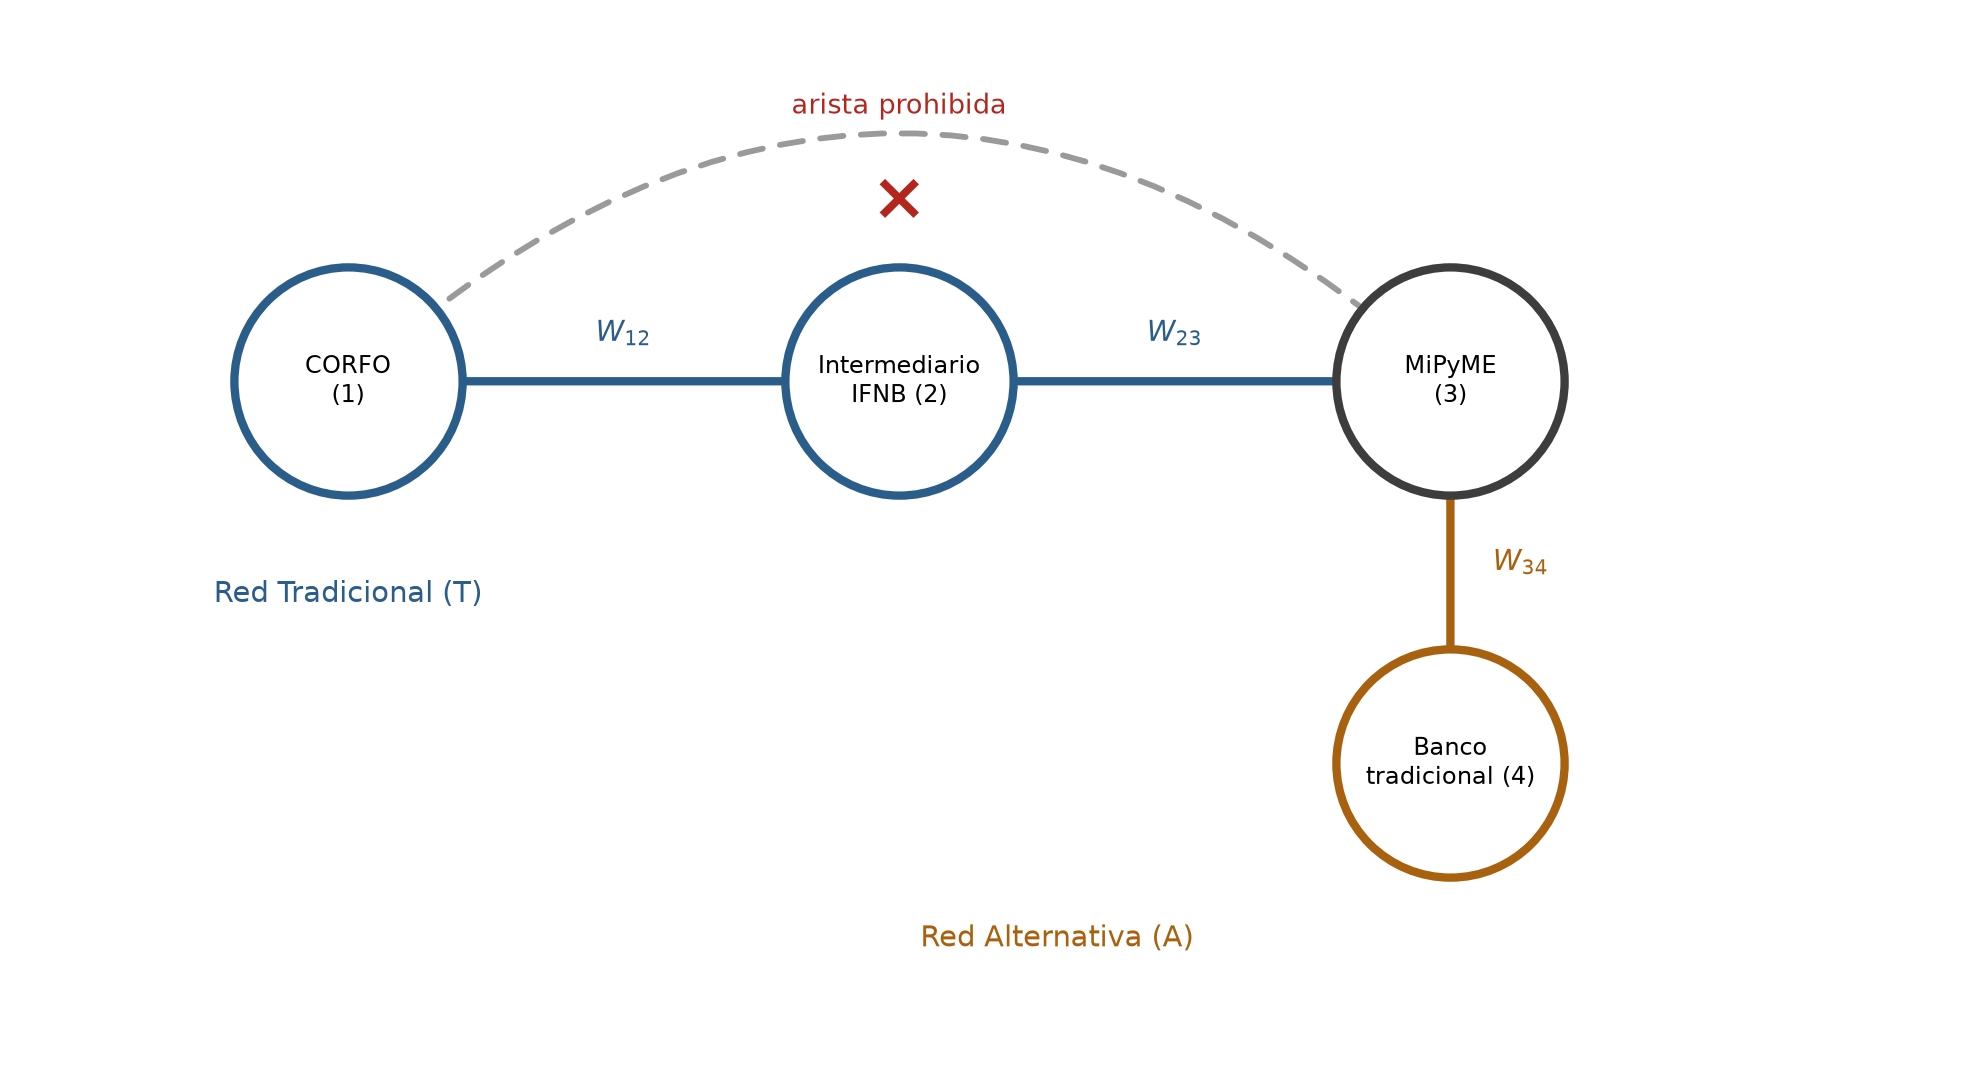
\includegraphics[width=0.85\textwidth]{diagrama_redes.png}
\caption{Estructura de las dos redes del caso de aplicación. La red Tradicional (azul) canaliza financiamiento de CORFO hacia la MiPyME a través de un intermediario financiero no bancario, con la arista directa CORFO--MiPyME prohibida. La red Alternativa (naranja) representa el acceso a crédito bancario de mercado. La MiPyME es el único agente presente en ambas redes.}
\label{fig:redes}
\end{figure}

\section{Notación}
\label{sec:notacion}

\begin{center}
\begin{tabular}{ll}
\hline
Símbolo & Significado \\
\hline
$W$ & Matriz simétrica de tamaños de contrato. $W_{ij}$ es el contrato vigente entre $i$ y $j$ \\
$P$ & Matriz antisimétrica de precios o pagos laterales entre pares de agentes \\
$M$ & Matriz de creencias de retorno esperado. $\mu_i = Me_i$ es el vector de creencias de $i$ \\
$\Sigma_i$ & Matriz de covarianza de retornos percibida por el agente $i$ \\
$\gamma_i$ & Coeficiente de aversión al riesgo del agente $i$ \\
$\Gamma$ & Matriz diagonal que agrupa los $\gamma_i$ de todos los agentes \\
$\Psi_i$ & Matriz que codifica qué contrapartes tiene permitidas el agente $i$ \\
$Q_i$ & Matriz de sensibilidad del agente $i$, definida como $\Psi_i^\top(2\gamma_i \Psi_i \Sigma_i \Psi_i^\top)^{-1}\Psi_i$ \\
$F$ & Conjunto de pares $(i,j)$ con $i<j$ donde el precio $P_{ij}$ puede ser no nulo \\
$Z_F$ & Matriz de coeficientes del sistema lineal que determina los precios (Teorema 1) \\
$\eta$ & Factor de amortiguación del algoritmo de negociación bilateral \\
$\lambda_A$ & Parámetro de fricción de acceso a la red Alternativa (modelo dual) \\
$\tau$ & Parámetro de transparencia o fricción del modelo dual \\
$m$ & Número de observaciones históricas por agente para estimar $\Sigma_i$ \\
$n$ & Número de agentes de la red. En este caso, $n=4$ \\
\hline
\end{tabular}
\end{center}

\section[Marco teórico. Elementos del modelo de Jalan y Chakrabarti]{Marco teórico. Elementos del modelo de \citeA{jalan_incentive-aware_2024} relevantes para la calibración empírica}

Esta sección recoge las definiciones y resultados de \citeA{jalan_incentive-aware_2024} directamente pertinentes para la etapa de aplicación a datos reales, dejando fuera los resultados de la Sección 3 del paper (fricciones, estática comparativa, detección de fuente) por no tener relación directa con el ejercicio de calibración de este hito.

\subsection{Factibilidad y estabilidad (Definiciones 2 y 3)}

Una tupla $(W,P)$ es factible si $W=W^\top$, $P=-P^\top$, y ambas obedecen las restricciones de red codificadas en $(\Psi_i)_{i\in[n]}$. Es estable si, además, cada agente $i$ maximiza su utilidad $g_i(W,P)$ dado $P$, sobre todas las alternativas factibles $W'$ que solo modifican su propia fila/columna. Estas dos definiciones son, por lo tanto, las que fijan qué significa formalmente un ``punto de equilibrio'' de la red CORFO--Intermediario--MiPyME--Banco, ya que $(W,P)$ es estable cuando ningún agente puede mejorar unilateralmente su utilidad renegociando sus contratos vigentes.

\subsection{Existencia y unicidad (Teorema 1)}

Bajo condiciones generales, el punto estable es único y se obtiene resolviendo el sistema lineal $Z_F \cdot \mathrm{uvec}(P)_F = \mathrm{uvec}(A-A^\top)_F$, donde $F$ es el conjunto de aristas permitidas y $Z_F$ se construye a partir de las matrices de sensibilidad $Q_i = \Psi_i^\top(2\gamma_i \Psi_i \Sigma_i \Psi_i^\top)^{-1}\Psi_i$. Este es, por lo tanto, el resultado que en principio permitiría, dado un conjunto de creencias $(M,\Gamma,\Sigma)$ como las declaradas en la Sección~\ref{sec:supuestos}, obtener un $W_{23}$ predicho por el modelo, cálculo que queda fuera del alcance de este hito y se deja como trabajo posterior.

\subsection{Negociaciones bilaterales (Algoritmo 1)}

En la práctica, el punto estable se alcanza mediante negociaciones bilaterales iterativas, en las que, en cada ronda, todos los pares de agentes permitidos actualizan simultáneamente su precio $P_{ij}$ hacia el valor que resuelve su desacuerdo, ponderado por un factor de amortiguación $\eta \in (0,1)$. El Teorema 4 establece que la convergencia está garantizada para $\eta < \eta^* = 2/\lambda_{\max}$, donde $\lambda_{\max}$ es el autovalor máximo de la matriz $(L^\dagger K)|_R$ construida a partir de las mismas matrices $Q_i$.

\subsection{Estimación con muestras finitas (Teorema 5)}
\label{sec:teorema5}

Todo lo anterior asume que cada agente conoce exactamente su matriz de covarianza $\Sigma_i$. Sin embargo, el Teorema 5 relaja este supuesto, mostrando que, si cada agente estima $\Sigma_i$ a partir de $m$ muestras independientes, el umbral de amortiguación estimado $\hat\eta^*$ satisface $\hat\eta^* \geq (1-o(1))\eta^*$ con probabilidad $1-\exp(-\Omega(n))$, siempre que $m \geq \lceil n\log n \rceil$. Es decir, el número de observaciones necesarias para que la estimación de covarianza no degrade sustancialmente el comportamiento del algoritmo de negociación crece solo levemente más rápido que linealmente con el número de agentes $n$ de la red.

Esta es, en consecuencia, la pieza teórica que Venegas nunca necesitó introducir en su tesis, precisamente porque trabajó con parámetros dados y no estimados. Para este trabajo, en cambio, dicho resultado define directamente un mínimo de datos históricos exigible antes de considerar defendible cualquier estimación de $\Sigma$ a partir de la red real.

\section{Datos disponibles y su método de obtención}
\label{sec:datos}

\subsection[Panel W12 (CORFO a Intermediario/IFNB)]{Panel $W_{12}$ (CORFO $\to$ Intermediario/IFNB)}

Se extrajo de las ``Cuentas Públicas Participativas'' anuales de CORFO (repositorio institucional \texttt{repositoriodigital.corfo.cl}, colección 2014--2024), permitió listar y descargar los PDF de cada gestión anual). De los 11 documentos descargados, se extrajo el monto de préstamos otorgados por CORFO a intermediarios financieros no bancarios (IFNB) para los años 2019, 2020 y 2024 (en 2016 solo se dispone de la cifra de colocaciones a MiPyMEs bajo el programa antecesor Microcrédito, sin el monto mayorista CORFO-IFNB desagregado). En cambio, para el resto de los años esta cifra desagregada no está publicada, y solo se dispone en algunos casos de la cifra agregada de ``colocaciones'' a MiPyMEs, que mezcla flujo nuevo con cartera rotativa (ver Sección~\ref{sec:limitaciones}).

\subsection[Ausencia de datos para W23 (Intermediario a MiPyME)]{Ausencia de datos para $W_{23}$ (Intermediario $\to$ MiPyME)}

No existe, hasta donde se ha buscado, una fuente pública que reporte esta arista de forma desagregada y comparable entre años. No obstante, el reglamento operativo del programa Crédito Corfo Mipyme (Texto Refundido, punto 19, ``Justificación de la utilización de los préstamos otorgados a los IFNB'') revela que CORFO sí recibe internamente, mes a mes y por operación individual, tanto la tasa de interés como el saldo de capital vigente de cada crédito, Dicha información resolvería directamente este vacío, aunque no es pública y solo sería accesible a través de un contacto institucional. Actualmente se encuentran en curso conversaciones con dicho contacto para evaluar su disponibilidad.

\subsection{Datos para la red Alternativa}

Se utilizan dos fuentes del Ministerio de Economía, ambas de acceso público. La primera es DIPRES, cuyo Informe de Monitoreo del programa 2020--2021 reporta la tasa de interés mayorista CORFO$\to$IFNB (4,23\%--4,73\% anual) y el spread de la tasa a cliente final IFNB respecto al benchmark de mercado ACHEF/EFA ($-7$ a $-10$ puntos porcentuales). La segunda es la ELE-7 (Séptima Encuesta Longitudinal de Empresas), cuyos microdatos completos (\texttt{ele7-full.csv}, 6.592 empresas) permiten obtener la tasa de interés del crédito de mayor monto aprobado en 2022 (variable \texttt{B066}), segmentada por tamaño de empresa (variable \texttt{TAMANO}) y anualizada según periodicidad reportada (variables \texttt{B067}/\texttt{B068}). Complementariamente, el informe oficial de resultados de la misma encuesta reporta la tasa de rechazo condicional a la solicitud de crédito por tamaño de empresa.

\section{Supuestos del modelo para las variables no observadas}
\label{sec:supuestos}

\subsection[Supuesto para W23. Tasa subsidiada del canal Tradicional]{Supuesto para $W_{23}$. Tasa subsidiada del canal Tradicional}

Se asume que la tasa de interés que los IFNB cobran a la MiPyME bajo el programa Crédito Corfo Mipyme se ubica entre 7 y 10 puntos porcentuales por debajo del benchmark de mercado (ACHEF/EFA), según reporta DIPRES en su Informe de Monitoreo 2020--2021 del programa. Tomando como benchmark de mercado la tasa mediana observada para empresas de menor tamaño (Sección~\ref{sec:tasa-mercado}), esto implica una tasa subsidiada implícita del orden de 3\%--6\% anual, cifra consistente en magnitud con la tasa mayorista CORFO$\to$IFNB (4,23\%--4,73\% anual, DIPRES 2021). Dado que ambas cifras coinciden en orden de magnitud, esta consistencia respalda el supuesto de que el IFNB traspasa el subsidio casi íntegro a la MiPyME, agregando solo un margen operativo menor, en línea con el rol de ``banca de segundo piso'' que describe CORFO para este programa.

\subsection[Supuesto para la red Alternativa. Tasa de mercado M34]{Supuesto para la red Alternativa. Tasa de mercado $M_{34}$}
\label{sec:tasa-mercado}

$M_{34}$ representa, en la notación del modelo, la creencia de retorno esperado entre la MiPyME y un banco tradicional si negociaran un contrato de crédito en la red Alternativa. No se dispone de una fuente que mida directamente esta creencia bilateral, por lo que se la aproxima mediante la tasa de interés de mercado efectivamente pagada por empresas de tamaño comparable, bajo el supuesto de que dicha tasa refleja razonablemente el costo/retorno que ambas partes anticiparían en una negociación real. Para la tasa de mercado que enfrentaría la MiPyME en el canal bancario tradicional (sin fondeo CORFO), se utiliza la tasa de interés anualizada del crédito de mayor monto aprobado en 2022, calculada directamente de los microdatos de la ELE-7 (variable B066 segmentada por TAMANO, con anualización explícita de los casos reportados en base mensual). Se reporta la mediana en preferencia a la media, dado que esta última se ve distorsionada por un pequeño número de casos atípicos en el segmento de empresas grandes, según se observa en la siguiente tabla.

\begin{center}
\begin{tabular}{lcc}
\hline
Tamaño (CORFO) & Tasa mediana anual 2022 & $n$ \\
\hline
Grande      & 10,43\% & 574 \\
Mediana     & 12,01\% & 225 \\
Pequeña 2   & 12,68\% & 150 \\
Pequeña 1   & 15,39\% & 151 \\
Micro       & 14,00\% & 152 \\
\hline
\end{tabular}
\end{center}

Se adopta, por lo tanto, el rango 14\%--15,4\% (segmentos Pequeña~1 y Micro) como supuesto de $M_{34}$ para la MiPyME en la red Alternativa. La tabla muestra una tendencia general de mayor tasa a menor tamaño (Grande 10,43\% frente a Pequeña~1 15,39\%); sin embargo, esta relación no es estrictamente monotónica, ya que Micro (14,00\%) queda levemente por debajo de Pequeña~1 (15,39\%). Dicha diferencia puede reflejar más bien el tamaño de muestra reducido ($n=151$ y $n=152$ respectivamente) que un efecto económico real, por lo que debe reportarse sin forzar una lectura estrictamente monotónica.

\subsection[Supuesto para la fricción de acceso lambda A]{Supuesto para la fricción de acceso $\lambda_A$}

$\lambda_A$ es, en el modelo dual de Venegas, el parámetro que determina cuán costoso o restringido resulta para la MiPyME acceder a la red Alternativa en comparación con la red Tradicional, y por lo tanto gobierna cómo la MiPyME reparte su portafolio entre ambos canales. Un $\lambda_A$ alto implica que, aun si el modelo predijera una tasa competitiva en la red Alternativa, la MiPyME en la práctica no podría aprovecharla con facilidad. Como segunda ancla, independiente de la anterior, se utiliza la tasa de rechazo condicional a la solicitud de crédito reportada en el informe oficial de resultados de la ELE-7, que llega a 15\% para MiPyMEs frente a 3\% para empresas grandes (cinco veces mayor). Adicionalmente, 111 de las 1.018 empresas que necesitaban crédito pero nunca lo solicitaron declaran autocensura, una población disjunta de las 819 empresas que sí solicitaron crédito. Esta brecha de acceso, combinada con la brecha de tasa anterior, sustenta por lo tanto el supuesto de que $\lambda_A$ es sustancialmente mayor que la fricción de acceso a la red Tradicional para el agente MiPyME.

\section{Relación entre los datos disponibles y el marco teórico}
\label{sec:relacion-teoria-datos}

\subsection{Aplicación del Teorema 5 al caso de cuatro agentes}

Con $n=4$ agentes (CORFO, Intermediario, MiPyME, Banco tradicional), el Teorema 5 exige un mínimo de $m \geq \lceil n\log n\rceil = \lceil 4\ln 4\rceil = 6$ observaciones independientes para que la estimación de $\Sigma$ no degrade sustancialmente la convergencia del algoritmo de negociación bilateral. Sin embargo, el panel real disponible para $W_{12}$ cubre únicamente 4 años, no consecutivos (2016, 2019, 2020, 2024), por debajo del umbral mínimo teórico.

\subsection{Relación con el Algoritmo 1 y el Teorema 4}

El Teorema 1 resuelve el punto estable de forma exacta mediante un sistema lineal, y para el caso de cuatro agentes con las restricciones estructurales ya conocidas ese sistema $Z_F$ es de baja dimensión, por lo que se resolvería exactamente y sin necesidad de iterar. En consecuencia, si más adelante se calcula un $W_{23}$ predicho a partir de los supuestos de este documento, el mecanismo directo sería el Teorema 1, y no el Algoritmo 1.

El Algoritmo 1, en cambio, cobra relevancia práctica en un problema distinto y de mayor escala, que es la implementación completa del modelo dual mediante la capa de acoplamiento T/A. Ahí, el sistema conjunto que resuelve la partición $w_3^T + w_3^A$ de la MiPyME se beneficia de un mecanismo descentralizado, en el que cada par de agentes negocia usando solo su propio precio vigente y sin necesidad de conocer de antemano toda la red, tal como lo haría un agente real. Es en ese contexto, y no en el cálculo puntual de este caso de cuatro agentes, donde el factor de amortiguación $\eta$ y su cota de convergencia (Teorema 4) pasan a ser relevantes en la práctica.

\section{Limitaciones}
\label{sec:limitaciones}

\begin{enumerate}
    \item Ambigüedad flujo/stock. En varios años, la cifra reportada de ``colocaciones'' a MiPyMEs mezcla desembolso nuevo con cartera rotativa de años anteriores, lo que impide tratarla como $W_{23}(t)$ en el sentido estricto del modelo, es decir, como una fotografía de contrato vigente.
    \item Asimetría de agregación entre redes. $W_{12}$ proviene de un programa e institución identificables, mientras que los supuestos de la red Alternativa provienen de promedios de mercado a nivel nacional (ELE-7), no de una relación bilateral banco--MiPyME específica.
    \item Identificabilidad estructural de $\Sigma_{13}$. La arista CORFO--MiPyME, al estar prohibida, deja esa entrada de covarianza débilmente identificada en cualquier intento de aplicar la Proposición 1 del paper, independientemente del volumen de datos disponible.
    \item Cobertura incompleta del panel CORFO. Existen años cuyos datos desagregados de este programa no están publicados. Esto significa que los años disponibles no son una muestra representativa del período completo, lo que introduce un sesgo de selección no cuantificado.
\end{enumerate}
